\chapter{Stato dell'Arte}
Questa Tesi si colloca nell'ambito del posizionamento ferrotramviario.\\*
Il posizionamento \`e un problema tipico del dominio ferroviario, tuttavia si presenta anche nel contesto ferrotramviario, poich\`e i sistemi ferrotramviari nascono come derivazione dai sistemi ferroviari.\\*
Al fine di introdurre gli argomenti trattati nel seguito della Tesi, in questo capitolo vengono brevemente introdotti i sistemi ferrotramviari, evidenziandone le principali differenze con i sistemi ferroviari. Si descrive infine lo stato dell'arte nell'ambito del posizionamento ferroviario e ferrotramviario.
\section{Sistemi Ferroviari e Ferrotramviari}
\`E possibile schematizzare un sistema ferroviario, o ferrotramviario, come un insieme di vetture vincolate a muoversi lungo una traccia fissata.\\*
Questa schematizzazione \`e, in grossolana approssimazione, valida per qualsiasi sistema ferroviario o ferrotramviario, a prescindere dal numero di veicoli transitanti o dall'estensione geografica. Ci\'o che invece differenzia un sistema ferroviario da un sistema ferrotramviario sono:
\begin{itemize}
		\item Le caratteristiche fisiche del veicolo transitante, come lunghezza e massa;
		\item Le caratteristiche geografiche dell'ambiente operativo;
		\item Gli scopi del trasporto.
\end{itemize}
In generale, nel trasporto ferroviario si utilizzano veicoli pesanti atti a trasportare persone o merci su lunghe percorrenze, pertanto \`e comune che l'ambiente operativo di un sistema ferroviario sia prevalentemente extra urbano.\\*
Nel trasporto ferrotramviario, di contro, si utilizzano veicoli leggeri per offrire un'alternativa al cittadino all'utilizzo di mezzi privati durante i suoi spostamenti all'interno di un'area metropolitana. Quest'ultima caratteristica implica che l'ambiente operativo di un sistema ferrotramviario sia radicalmente diverso dall'ambiente operativo di un sistema ferroviario. Le vetture si muovono lungo traccie installate su strade urbane, e di conseguenza il traffico ferrotramviario condivide l'ambiente con il traffico cittadino, come mostrato in figura \ref{fig:tramschema}.\\*
\begin{figure}[h]
		\centering
		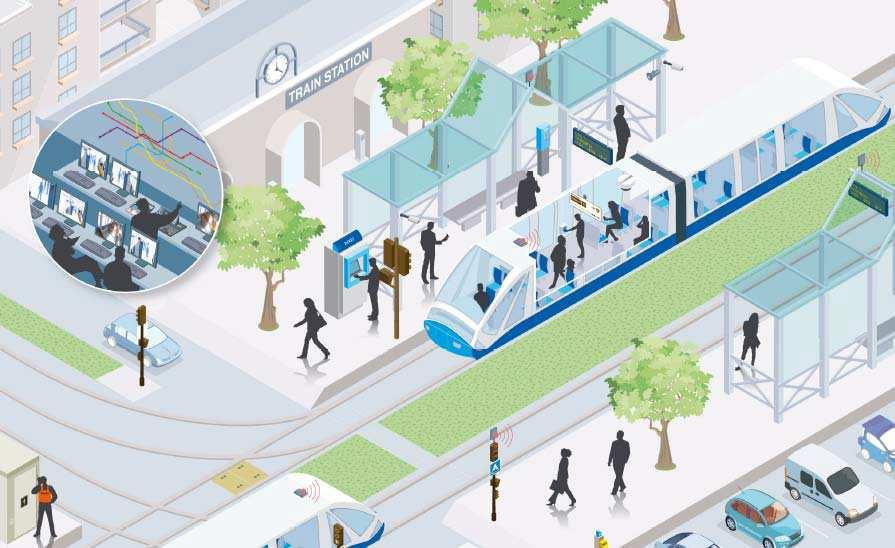
\includegraphics[width=0.7\linewidth]{img/twschema}
		\caption{Schema di un tipico scenario ferrotramviario}
		\label{fig:tramschema}
\end{figure}
\section{Il problema del posizionamento}
Per posizionamento ferroviario si intende la valutazione della posizione di un treno all'interno di una traccia ferroviaria. Tale posizione viene espressa come progressiva chilometrica rispetto a una posizione nota, come ad esempio l'origine della linea. \cite{trainpositioning}\\*
\subsubsection{Odierne Tecniche di Posizionamento}
Gli odierni sistemi di posizionamento si basano principalmente sull'utilizzo di strumenti installati a terra, chiamati \emph{beacon}, o \emph{balise} in gergo ferroviario, i quali hanno lo scopo di rilevare il passaggio di un treno.\cite{tecnicheodierne}
Esiste uno standard a livello europeo al quale gli odierni sistemi di posizionamento si devono uniformare, l' \emph{European Train Control System} (ETCS).\\*
Nel corso della storia, ogni paese europeo ha sviluppato autonomamente le proprie infrastrutture ferroviarie e relative regole operative. Tuttavia, ad oggi i treni possono attraversare le frontiere, pertanto \`e necessario sviluppare un sistema ferroviario standard che rispetti una comune normativa operazionale europea. Tale sistema prende il nome di \emph{European Rail Traffic Management System} (ERTMS) \cite{ertms}, ed ETCS \`e il sottosistema di ERTMS dedicato al posizionamento delle vetture.\\*
Come standard, ETCS definisce specifici livelli di \emph{compliance} che possiede un sistema di posizionamento rispetto ad ETCS, ed essi vanno dal livello \texttt{ETCS-0} al livello \texttt{ETCS-3}. \cite{svolta}
\\*
L'obiettivo \`e quello di sviluppare progressivamente un sistema di posizionamento completamente autonomo (\texttt{ETCS-3}), partendo da un sistema interamente \emph{non-compliant} con ETCS (\texttt{ETCS-0}).
\\*
Allo stato attuale, quasi tutti i sistemi di posizionamento sono \texttt{ETCS-2}. Nei livelli \texttt{ETCS-1} e \texttt{ETCS-2}, le traccie vengono suddivise in blocchi, e all'entrata di ciascun blocco viene posizionato un \emph{beacon} in grado di rilevare la presenza di un treno.\\*
L'autorizzazione all'ingresso in un blocco viene rilasciata se nessun altro treno sta occupando il blocco al quale si vuole accedere, mentre un sistema di \emph{odometria} installato a bordo, posiziona il treno rispetto all'ultimo \emph{beacon} incontrato.\\*
Nel livello \texttt{ETCS-3}, non sono richiesti segnali provenienti dalla linea: un treno deve essere in grado di posizonarsi autonomamente. \cite{etcs3}\\*
In sintesi, i livelli ETCS possono essere descritti come segue:
\begin{itemize}
	\item \texttt{ETCS-0}: Sistema non conforme a ETCS;
	\item \texttt{ETCS-1}: Utilizzo di apparati di posizionamento installati a terra, autorizzazione a procedere segnalata al macchinista attraverso indicazioni semaforiche;
	\item \texttt{ETCS-2}: Come \texttt{ETCS-1}, ma l'autorizzazione a procedere \`e gestita da un sistema automatico di scambio, denominato sistema di \emph{interlocking};\cite{interlocking}
	\item \texttt{ETCS-3}: Posizionamento autonomo, nessun utilizzo di apparati a terra.
\end{itemize}
\begin{figure}[h]
	\centering
	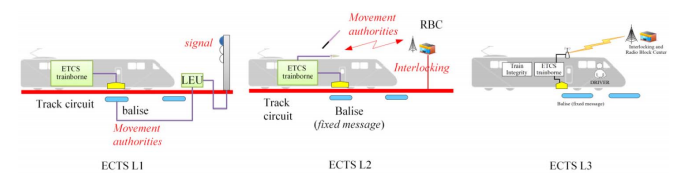
\includegraphics[width=\linewidth]{img/etcs123.png}
	\caption{Livelli \texttt{ETCS}}
	\label{fig:etcs123}
\end{figure}
Il livello \texttt{ETCS-2} prevede che l'autorizzazione a procedere venga gestita dal sistema di \emph{interlocking} e non dal solo operatore umano notificato mediante indicazioni semaforiche.\\*
La funzionalit\`a offerta del sistema di \emph{interlocking} viene pertanto considerata \emph{safety-critical}, in quanto un suo fallimento pu\`o portare a conseguenze anche catastrofiche.\cite{marocchini}\\*
ETCS adotta un approccio incrementale alla realizzazione di sistemi di posizionamento autonomi. Un sistema di posizionamento \texttt{ETCS-3} deve continuare a interagire con il sistema di \emph{interlocking}, quindi deve essere considerato a sua volta un sistema \emph{safety-critical}.\\*
L'implementazione hardware e software di un sistema \texttt{ETCS-3} viene dunque vincolata da standard generici per sistemi \emph{safety-critical} \cite{MISRA} \cite{sil}, e da standard specifici del dominio ferroviario \cite{50128}.\\*
ERTMS/ETCS \`e pensato per sistemi ferroviari, mentre nel dominio ferrotramviario vige la regola della \emph{marcia a vista}. Il rispetto di ETCS non \`e obbligatorio in detto contesto, tuttavia le tecniche di posizionamento ivi utilizzate rispettano spesso le linee guida imposte da ETCS. 
\section{Verso ETCS-3}
Gli attuali sistemi di posizionamento richiedono un minimo intervento di computer installati a bordo e una grande quantit\`a di apparati installati a terra. Gli apparati di terra sono costosi e hanno un impatto ambientale non trascurabile, pertanto \`e necessario iniziare a pianificare una migrazione verso sistemi \texttt{ETCS-3}.\cite{market}\\*
Il sistema oggetto della Tesi \`e un sottosistema di posizionamento conforme alla filosofia \texttt{ETCS-3}.\\*
Nell'ottica di voler realizzare un sistema di posizionamento autonomo, il treno viene modellato come un \emph{Cyber-Physical System} (CPS).\\*
Un CPS \`e un sistema che consiste di un computer (sottosistema \emph{cyber}) e un oggetto da esso controllato (sottosistema \emph{physical}).
Il sottosistema \emph{cyber} \`e essenzialmente un elaboratore che opera in un tempo discreto, dispone di processore, memoria, e di interfacce I/O che abilitano l'interazione del CPS con eventuali operatori umani.\\*Il sottosistema \emph{physical} consiste di un sistema governato dalle leggi della fisica che opera in un tempo continuo.
\cite{cps}\cite{cecca}\\*
Nella fattispecie, l'oggetto controllato \`e il treno, mentre l'elemento \emph{cyber} \`e costituito da un \emph{sistema di sistemi} composto da un'unit\`a in grado di campionare e processare un certo insieme di misure, e da un'unit\`a in grado di controllare il movimento del treno. Quest'ultima unit\`a prende il nome di \emph{On Board Control Unit} (OBCU), ed \`e il computer di bordo nominale che ogni treno deve possedere in accordo a ERTMS/ETCS.\\*
Lo scopo della Tesi \`e quello di mostrare i risultati sperimentali delle campagne di analisi condotte sul sottosistema \emph{cyber} del CPS descritto.\\*
Tale sottosistema ha lo scopo di stimare la posizione di un treno attraverso l'uso combinato di un insieme di sensori installati a bordo.\\*
I valori campionati dai sensori dovranno essere integrati al fine di ottenere una stima sicura e affidabile della posizione del treno. Tale integrazione viene realizzata grazie all'utilizzo di un algoritmo noto come \emph{Sensor Fusion Algorithm} (SFA). \cite{sfarailway} 